\documentclass[12pt]{article}
\usepackage{times,amssymb,amsmath,cite,graphicx}
\usepackage{graphicx,ifpdf,hyperref,color,wasysym,colortbl,}
\usepackage{amsmath,alltt,epsfig,xspace,theorem,changebar,textcomp,amssymb}

%% Package for drawing figures
\usepackage{tikz}
\usetikzlibrary{arrows}
\usetikzlibrary{calc}
\usetikzlibrary{decorations.markings}
\usetikzlibrary{decorations.pathmorphing}
\usetikzlibrary{decorations.pathreplacing}
\usetikzlibrary{matrix}
\usetikzlibrary{trees}
\usepackage{pgfplots}
\usepackage{subfigure}
\usepackage{skak}

\setlength{\oddsidemargin}{.25in}
\setlength{\evensidemargin}{.25in}
\setlength{\textwidth}{6in}
\setlength{\topmargin}{-0.4in}
\setlength{\textheight}{8.5in}

\author{Benjamin Walker}
\title{Interactive Proof Systems}
\date{\today{}}

\begin{document}

\maketitle

\section{Introduction}

An interactive proof system presents a unique way to assert that a given string does or does not belong to a certain language. Interactive proofs (IP) have enormous relevance in the computational world. They are built on top of probabilistic polynomial verifiers and are used largely in cryptology, approximation algorithms, and have a future ahead of them helping verify other difficult problems in PSPACE. Sipser defined interactive proof systems as "systems [that] provide a way to define a probabilistic analog of the class NP, much as the probabilistic polynomial time algorithms provide a probabilistic analog of P." \cite{sipser}

\section{Introducing Provers and Verifiers}
To start introducing what an interactive proof system is, it is important to establish a common definition of what Provers and Verifiers are.

The role of a Prover is to convince the Verifier of some claim it has. The point of IP is to verify truth, not to solve it. The Prover has no computational constraints. The Prover by definition is capable of solving any problem presented to it. The Verifier has the role of establishing a high level of acceptance for what the Prover communicates to it. In other words, the Verifier verifies the truthfulness of the Prover's claim. The Verifier is bounded by polynomial computational constraints; had it not been so, the Verifier could solve all of the problems itself, and there would be no need for a Prover. The Prover and Verifier definition is not yet complete. To illustrate why more is needed, there will be first given examples of problems to set the stage for a more complicated problem that the current definitions are not sufficient for. A full definition of what an IP consists of will be covered later in this paper.

\subsection{SAT}
The NP-Complete SAT problem is used to illustrate these definitions. Suppose that the IP was given a SAT problem with several variables:

$SAT \equal (\overline{a} \vee \overline{b} \vee c \vee k \vee \overline{u}) \wedge (a \vee \overline{g}) 
\wedge ... \wedge (r \vee \overline{y} \vee z)$

It is the Prover's job to find an answer to this problem and try to convince the polynomial constricted Verifier of the accuracy of the presented solution. In this example, a set of variables with their associated boolean values could simply be presented to the Verifier:

\begin{center}
\begin{tabular}{|l|c|c|c|c|c|c|c|c|c|}
\hline
  a & b & c & g & k & ... & r & u & y & z \\
   &     &     &     &     &     &     &     &     & \\
\hline
  0  &  0  &  1  &  0  &  0  & ... &  1  &  0  &  0  &  1 \\
      &     &     &     &     &     &     &     &     & \\
\hline
  \end{tabular}
\end{center}

The Prover would pass a solution (as is seen in the table above) to the Verifier. It is then the Verifier's job to assert, within polynomial time, the validity of the answer provided. The Verifier can simply do this by entering the boolean values it received from the Prover directly into the SAT problem. The Verifier will not take more than polynomial time to compute. If the problem returns true, the Verifier has been convinced.

\subsection{Verifying Correct Isomorphic Relationships}
Using this same, incomplete, definition of what a Prover and a Verifier is, the example of validating a relationship between two isomorphic graphs is given. The graph isomorphic problem is a typical example used for introducing interactive proof systems, because this problem has not been proved to be in the P or NP-Complete class.

Two graphs are provided below for verifying an isomorphic relationship, $Graph H$ and $Graph G$ respectively: 

\begin{tikzpicture}
[nodedecorate/.style={shape=circle,inner sep=3pt,draw,thick},%
  linedecorate/.style={-,thick}]
%% nodes or vertices
\foreach \nodename/\x/\y/\direction/\navigate in {2/1/3/above/north,
  1/0/4/above/north, 3/3/2.5/above/north, 4/3/1.5/below/south,
  5/1/1/below/south, 7/-2/2/left/west, 6/0/0/below/south, 8/8/2/above/north, 
  9/0/2/left/west, 10/-2/4/above/north, 11/-2/0/below/south}
{
  \node (\nodename) at (\x,\y) [nodedecorate] {};
  \node [\direction] at (\nodename.\navigate) {$\nodename$};
}
%% edges or lines
\path
\foreach \startnode/\endnode in {1/2, 1/5, 2/3, 2/5, 2/7, 3/4, 3/5,
  4/6, 5/6, 6/7, 10/1, 10/7, 11/7, 11/6, 8/1, 8/6, 8/5, 8/2, 9/2, 9/5}
{
  (\startnode) edge[linedecorate] node {} (\endnode)
};
\end{tikzpicture}
\\[5pt]
\begin{tikzpicture}
[nodedecorate/.style={shape=circle,inner sep=3pt,draw,thick},%
  linedecorate/.style={-,thick}]
%% nodes or vertices
\foreach \nodename/\x/\y/\direction/\navigate in {2/6/2/above/north,
  1/5/0.8/below/east, 3/3/2/above/north, 4/0.5/1.5/above/north,
  5/8/0/below/south, 7/3/1.5/below/south, 6/1/0.5/below/south, 8/7/1.25/above/north, 
  9/8/1.75/right/east, 10/4/0/below/south, 11/0/1/below/south}
{
  \node (\nodename) at (\x,\y) [nodedecorate] {};
%  \node [\direction] at (\nodename.\navigate) {$\nodename$};
}
%% edges or lines
\path
\foreach \startnode/\endnode in {1/2, 1/5, 2/3, 2/5, 2/7, 3/4, 3/5,
  4/6, 5/6, 6/7, 10/1, 10/7, 11/7, 11/6, 8/1, 8/6, 8/5, 8/2, 9/2, 9/5}
{
  (\startnode) edge[linedecorate] node {} (\endnode)
};
\end{tikzpicture}

The Prover takes both $Graph G$ and $Graph H$ and figures out that they are indeed isomorphic. The Verifier is more than capable of verifying the isomorphic relationship between the two graphs. The data that the Prover sends to the Verifier could be a list of nodes of $Graph H$ with its associating vertex neighbors connected by an edge. This list is compared to $Graph G$. To settle the curious mind that $Graph G$ and $Graph H$ above are isomorphic, $Graph H$ is provided below with its associating isomorphic node assignment.

\begin{tikzpicture}
[nodedecorate/.style={shape=circle,inner sep=3pt,draw,thick},%
  linedecorate/.style={-,thick}]
%% nodes or vertices
\foreach \nodename/\x/\y/\direction/\navigate in {2/6/2/above/north,
  1/5/0.8/below/east, 3/3/2/above/north, 4/0.5/1.5/above/north,
  5/8/0/below/south, 7/3/1.5/below/south, 6/1/0.5/below/south, 8/7/1.25/above/north, 
  9/8/1.75/right/east, 10/4/0/below/south, 11/0/1/below/south}
{
  \node (\nodename) at (\x,\y) [nodedecorate] {};
  \node [\direction] at (\nodename.\navigate) {$\nodename$};
}
%% edges or lines
\path
\foreach \startnode/\endnode in {1/2, 1/5, 2/3, 2/5, 2/7, 3/4, 3/5,
  4/6, 5/6, 6/7, 10/1, 10/7, 11/7, 11/6, 8/1, 8/6, 8/5, 8/2, 9/2, 9/5}
{
  (\startnode) edge[linedecorate] node {} (\endnode)
};
\end{tikzpicture} 

\section{Formal  Definition of IP}
We have shown that a Prover can convince the Verifier of a correct answer in polynomial time, but can the Prover prove to the Verifier that an incorrect answer is not correct in polynomial time?

Interestingly, yes, provided the Prover and Verifier definitions can be expanded. Among the key parts of what makes an IP is the communication that can occur between the Prover and Verifier. The Verifier is allowed to ask the Prover questions as many times as it sees fit. The Verifier is also allowed to be a probabilistic polynomial time machine rather than just a normal polynomial verifier.

This definition of a Prover and a Verifier is what makes an interactive proof system. Written more succinct:

\begin{center}
\begin{tabular}{ c c }
{\LARGE Prover} & {\LARGE Verifier} \\
%% \pause
Convince the Verifier & Verify the answer \\
No computational constraints & Polynomial time only \\
Can engage in a two-way & Allowed to be a probabilistic \\
dialog with the Verifier & polynomial time machine \\
\end{tabular}
\end{center}

\subsection{Verifying Incorrect Isomorphic Relationships}

The reason the Isomorphic Graphs problem was chosen is because they are ''elusive". Elusive problems are categorized as problems in the class NP that are not known to be in P or to be in NP-Complete. These elusive problems, among other difficult problems, present a good illustration of what an IP can do and was originally meant for.

Using $Graph G$ and (a new) $Graph H$ below, the Prover discovered that these two graphs are not isomorphic and is determined to convince the Verifier.

\begin{tikzpicture}
[nodedecorate/.style={shape=circle,inner sep=3pt,draw,thick},%
  linedecorate/.style={-,thick}]
%% nodes or vertices
\foreach \nodename/\x/\y/\direction/\navigate in {2/1/3/above/north,
  1/0/4/above/north, 3/3/2.5/above/north, 4/3/1.5/below/south,
  5/1/1/below/south, 7/-2/2/left/west, 6/0/0/below/south, 8/8/2/above/north, 9/0/2/left/west, 10/-2/4/above/north, 11/-2/0/below/south}
{
  \node (\nodename) at (\x,\y) [nodedecorate] {};
  \node [\direction] at (\nodename.\navigate) {$\nodename$};
}
%% edges or lines
\path
\foreach \startnode/\endnode in {1/2, 1/5, 2/3, 2/5, 2/7, 3/4, 3/5,
  4/6, 5/6, 6/7, 10/1, 10/7, 11/7, 11/6, 8/1, 8/6, 8/5, 8/2, 9/2, 9/5}
{
  (\startnode) edge[linedecorate] node {} (\endnode)
};
\end{tikzpicture}
\\[5pt]
\begin{tikzpicture}
[nodedecorate/.style={shape=circle,inner sep=3pt,draw,thick},%
  linedecorate/.style={-,thick}]
%% nodes or vertices
\foreach \nodename/\x/\y/\direction/\navigate in {2/-2/2/above/north,
  1/0.5/0.5/below/east, 3/4/2/above/north, 4/5/2/above/north,
  5/6/0/below/south, 7/-1.25/1/left/west, 6/1/1/above/north, 
  8/-2/0/below/south, 9/8/1/above/north, 11/-0.75/0.75/left/south, ?/7/1.35/above/north}
{
  \node (\nodename) at (\x,\y) [nodedecorate] {};
%%  \node [\direction] at (\nodename.\navigate) {$\nodename$};
}
%% edges or lines
\path
\foreach \startnode/\endnode in {1/2, 1/5, 2/3, 2/5, 2/7, 3/4, 3/5,
  4/6, 5/6, 6/7, 11/7, 11/6, 8/1, 8/6, 8/5, 8/2, 9/2, 9/5, ?/4, ?/9}
{
  (\startnode) edge[linedecorate] node {} (\endnode)
};
\end{tikzpicture}

The Verifier, having been told that these graphs are not isomorphic chooses one of the two graphs at random. Suppose $Graph H$ was chosen. The Verifier creates a new graph, $Graph J$, isomorphic to $Graph H$. {\em Note: Mixing the location of the nodes, while keeping the edges between vertices is a polynomial time event; thus the Verifier can do this.} The Prover is provided $Graph J$ and is requested to identify which graph $Graph J$ came from. If the Prover really did figure out that the graphs were not isomorphic, then it will always respond with the correct graph. Playing the pessimist, the Verifier is aware that the Prover could have guessed where $Graph J$ came from, and it had a 50\% chance to get it right. The Verifier is not yet convinced that the Prover knows that the graphs are not isomorphic, so this discussion continues to happen. The Verifier selects at random one of the two original graphs, mixes the vertices and the Prover is supposed to tell the Verifier which graph it came from for a second time. 

Every time the Prover provides an answer to the Verifier, the Verifier becomes 50\% more certain that the Prover is telling the truth. $1 - \frac{1}{2^n}$ is a representation of what percentage the Verifier is completely convinced, where $n$ is the number of times that the Prover and the Verifier have communicated. The Verifier will never truly be 100\% certain that the Prover is telling the truth, so there is an arbitrary threshold of how sure the Verifier needs to be in order to be convinced of the Prover's initial claim.

Again, to satisfy the curious mind, the non-isomorphic $Graph H$ has been provided below with it's nodes assigned:

\begin{tikzpicture}
[nodedecorate/.style={shape=circle,inner sep=3pt,draw,thick},%
  linedecorate/.style={-,thick}]
%% nodes or vertices
\foreach \nodename/\x/\y/\direction/\navigate in {2/-2/2/above/north,
  1/0.5/0.5/below/east, 3/4/2/above/north, 4/5/2/above/north,
  5/6/0/below/south, 7/-1.25/1/left/west, 6/1/1/above/north, 
  8/-2/0/below/south, 9/8/1/above/north, 11/-0.75/0.75/left/south, ?/7/1.35/above/north}
{
  \node (\nodename) at (\x,\y) [nodedecorate] {};
  \node [\direction] at (\nodename.\navigate) {$\nodename$};
}
%% edges or lines
\path
\foreach \startnode/\endnode in {1/2, 1/5, 2/3, 2/5, 2/7, 3/4, 3/5,
  4/6, 5/6, 6/7, 11/7, 11/6, 8/1, 8/6, 8/5, 8/2, 9/2, 9/5, ?/4, ?/9}
{
  (\startnode) edge[linedecorate] node {} (\endnode)
};
\end{tikzpicture}


% \begin{center}
% \begin{tabular}{|l|c|c|c|c|c|c|c|c|}
% \hline
%   Current & 111 & 110 & 101 & 100 & 011 & 010 & 001 & 000 \\
%   pattern &     &     &     &     &     &     &     & \\
% \hline
%   New cell &  0  &  0  &  0  &  0  &  1  &  0  &  0  &  1 \\
%   state    &     &     &     &     &     &     &     & \\
% \hline
%   \end{tabular}
% \end{center}

% \begin{itemize}
% \item[Class 1:] Nearly all initial patterns evolve quickly into a
% \end{itemize}

\section{More Directions of IP}

So far the basic definition of what an IP consists of has been covered; however, interactive proofs have a very large extension into the field of advanced computation. This paper is not meant to delve deeply into the applications that IP can go, but here are some of the most prominent purposes of why we use IP.

\subsection{Zero Knowledge}

Cryptology has been largely effected by IP. Zero Knowledge is a process by which the Verifier is convinced without receiving any relevant information to the problem that the Prover claims a solution to \cite{zk}. How can this be? Cryptology is all about obtaining and verifying authenticity without giving any relevant information. Because IP allows this kind of communication, cryptology has become more secure.

Hamilton Circuits give a great illustration on how this ''Zero Knowledge" IP can work. Suppose $Graph G$ is claimed to contain a Hamilton Circuit by the Prover, but the Prover doesn't want to give the circuit path to the Verifier. The Prover will create a second graph, $H$, and claim that it is isomorphic to $Graph G$. If what the Prover says is true, then $Graph H$ also contains a Hamilton Circuit. The Verifier can ask for either the isomorphic relationship between $Graph G$ and $Graph H$, or the Verifier can ask for the Hamilton Circuit in $Graph H$, but not both for the same graph. The Prover would create a new supposedly isomorphic graph to $Graph G$ every time that the Verifier wants to test the Prover. Both isomorphic graphs and Hamilton Circuits are verifiable in polynomial time. In order for the Verifier to assert that $Graph G$ really does contain a Hamilton Circuit, the Verifier would need the isomorphic relationship and the Hamilton Circuit in $Graph H$. Hence, by the same probabilistic measure mentioned before: $1 - \frac{1}{2^n}$, the Verifier can assert that the Prover does indeed know of a Hamilton Circuit in $Graph G$.

\subsection{PSPACE = IP}

It turns out that an IP can be made for every single language in PSPACE. Sipser proves this by showing that IP is a subset of PSPACE and that PSPACE is a subset of IP \cite{sipser}. The original discovery of IP lead mathematicians to believe that the usefulness was more limited to ''elusive" problems. Thankfully this is not the case. Because PSPACE = IP, IP can be used in depth in almost all advanced areas of computational theory. This means that an IP problem can be created to verify any string in every language in PSPACE.

\subsection{Multiprover Interactive Proofs}
Multiprover interactive proofs (MIP) is exactly what it sounds like. It's the same thing as a normal IP except there can be more than one prover. To visualize the usefulness of MIP, imagine an interrogator as the Verifier, and there has been a group of people suspected of doing a heist together. Those being interrogated (the Provers) are trying to convince the interrogator that they had nothing to do with the heist. Those interrogated are kept in separate rooms; thus, there is no communication between them once the interrogation has begun. If the interrogator asks a circumstantial question to the first suspect and doesn't believe him, he can move on to the second, third, or fourth suspect and ask the same questions. If there is a discrepancy between answers, then the interrogator is not convinced \cite{ips}. It is much easier to verify the truthfulness of the Prover's claim by asking another Prover.

IP is naturally a subset of MIP, because MIP can simply ignore all of the Provers except for one and act like an IP. MIP is then at least as large as PSPACE. In fact Travis Hance has shown that $NEXP \subseteq MIP$ \cite{mip}. This means that a MIP can be created to verify a string for every single language in exponential space. 

\section{Conclusion}

Mathematicians are just breaking the surface of the potential for interactive proof systems. IP is used in approximation algorithms, cryptology, graph problems, and everything else in PSPACE. The unlimited communication between the Prover and the Verifier combined with the probabilistic polynomial verifier is what makes the interactive proof system so powerful. IP is indeed one of the most important aspects of computational theory.

\bibliographystyle{acm}
\bibliography{bibliography}

\end{document}
